% answers.tex -- marking criteria and sample answers for questions.tex (Module 6 short answer).
% NESA marking-guideline style: a criteria table for each part, then a sample answer.
% Every number: checks/m6-short-answer/numbers.py
% Build: TEXINPUTS=.: xelatex answers.tex (twice)
\documentclass[12pt]{article}
\usepackage{quiz}
\hypersetup{pdftitle={Short Answer Questions - Module 6 - Electromagnetism - Marking guidelines}}
% links between the two PDF files are not possible, so question headings are plain text here
\renewcommand\hyperlink[2]{#2}
\newcommand\anstopic[1]{\par\Needspace{8\baselineskip}\vspace{4mm}%
  \begin{center}{\headfont\bfseries\fontsize{14}{18}\selectfont #1\par}\end{center}\vspace{2pt}}

\begin{document}
\quiztitle{Year 12 Physics}{Short Answer Questions - Module 6 - Electromagnetism:\\
  Marking Guidelines and Sample Answers}

Data used: $e = \qty{1.602e-19}{C}$, $m_\mathrm{e} = \qty{9.109e-31}{kg}$, $m_\mathrm{p} = \qty{1.673e-27}{kg}$,
$\mu_0 = 4\pi\times10^{-7}\,\si{N.A^{-2}}$, $g = \qty{9.8}{m.s^{-2}}$. In calculations, a correct answer
from a correct method with an earlier error carried forward still earns the later marks.

% =====================================================================
\anstopic{Topic 1 - Charged Particles in Electric and Magnetic Fields}

% ---- Q1
\ansq
\anspart{a}
\begin{crit}
  \critrow{Correctly calculates the electric field strength}{1}
\end{crit}
\sample
$E = \dfrac{V}{d} = \dfrac{500}{0.040} = \qty{1.25e4}{V.m^{-1}}$.
\anspart{b}
\begin{crit}
  \critrow{Correctly calculates the acceleration}{1}
\end{crit}
\sample
$a = \dfrac{F}{m} = \dfrac{qE}{m} = \dfrac{(\num{1.602e-19})(\num{1.25e4})}{\num{9.109e-31}} = \qty{2.2e15}{m.s^{-2}}$.
\anspart{c}
\begin{crit}
  \critrow{Correctly calculates the speed}{2}
  \critrow{Uses $qV = \frac{1}{2}mv^2$ (or $v^2 = u^2 + 2as$)}{1}
\end{crit}
\sample
Work done by the field $=$ gain in kinetic energy: $qV = \frac{1}{2}mv^2$, so
\[ v = \sqrt{\frac{2qV}{m}} = \sqrt{\frac{2(\num{1.602e-19})(500)}{\num{9.109e-31}}} = \qty{1.33e7}{m.s^{-1}} \]

% ---- Q2
\ansq
\anspart{a}
\begin{crit}
  \critrow{Correctly calculates the vertical distance}{3}
  \critrow{Calculates the acceleration AND the time between the plates}{2}
  \critrow{Calculates the field strength, the acceleration or the time}{1}
\end{crit}
\sample
$E = \dfrac{150}{0.020} = \qty{7500}{V.m^{-1}}$, so
$a = \dfrac{eE}{m} = \dfrac{(\num{1.602e-19})(7500)}{\num{9.109e-31}} = \qty{1.32e15}{m.s^{-2}}$ (towards the
positive plate). The horizontal velocity is constant, so the time between the plates is
$t = \dfrac{0.060}{\num{2.0e7}} = \qty{3.0e-9}{s}$.
\[ s_y = \tfrac{1}{2}at^2 = \tfrac{1}{2}(\num{1.32e15})(\num{3.0e-9})^2 = \qty{5.9e-3}{m} \;(\qty{5.9}{mm}, \text{ upwards}) \]
This is less than the \qty{10}{mm} to the top plate, so the electron leaves the plates without hitting
them.
\anspart{b}
\begin{crit}
  \critrow{Gives a correct similarity AND a correct difference}{2}
  \critrow{Gives a correct similarity OR difference}{1}
\end{crit}
\sample
Similar: in both cases a constant force acts at right angles to the initial velocity. The velocity
along the plates (horizontal) stays constant, while the perpendicular velocity increases steadily, so
both paths are parabolas. Different: the electron's acceleration ($\qty{1.3e15}{m.s^{-2}}$, towards the
positive plate, here upwards) is far larger than $g$, and it depends on the charge and mass of the
particle; gravity on the electron is negligible.

% ---- Q3
\ansq
\anspart{a}
\begin{crit}
  \critrow{States that the magnetic force provides the centripetal force AND rearranges correctly}{2}
  \critrow{Writes $qvB = \frac{mv^2}{r}$}{1}
\end{crit}
\sample
The magnetic force is always at right angles to the velocity, so it provides the centripetal force:
$qvB = \dfrac{mv^2}{r}$. Dividing by $v$ and rearranging: $r = \dfrac{mv}{qB}$.
\anspart{b}
\begin{crit}
  \critrow{Correctly calculates the radius}{1}
\end{crit}
\sample
$r = \dfrac{(\num{1.673e-27})(\num{4.0e6})}{(\num{1.602e-19})(0.25)} = \qty{0.17}{m}$.
\anspart{c}
\begin{crit}
  \critrow{Explains that the force is at right angles to the velocity, so it does no work}{1}
\end{crit}
\sample
The magnetic force is always at right angles to the velocity, so it does no work. It changes the
direction of the velocity but not the speed, so the kinetic energy is constant.

% ---- Q4
\ansq
\anspart{a}
\begin{crit}
  \critrow{Explains that the electric and magnetic forces are opposite and balance only when $qE = qvB$,
    AND calculates $v$}{2}
  \critrow{Explains the balance OR calculates $v$}{1}
\end{crit}
\sample
In the selector, the electric force $qE$ and the magnetic force $qvB$ act in opposite directions. The
electric force does not depend on speed, but the magnetic force does, so they balance only at one
speed: $qE = qvB$, so $v = \dfrac{E}{B} = \dfrac{\num{2.0e4}}{0.10} = \qty{2.0e5}{m.s^{-1}}$. Slower ions
are deflected by the electric force; faster ions by the magnetic force.
\anspart{b}
\begin{crit}
  \critrow{Correctly calculates the mass}{2}
  \critrow{Uses $r = \frac{mv}{qB}$ with correct values}{1}
\end{crit}
\sample
$r = \dfrac{mv}{qB}$, so $m = \dfrac{qBr}{v} = \dfrac{(\num{1.602e-19})(0.20)(0.24)}{\num{2.0e5}} =
\qty{3.8e-26}{kg}$ (about 23 atomic mass units: a sodium ion).
\anspart{c}
\begin{crit}
  \critrow{States that they land further from the entrance, because $r = \frac{mv}{qB}$ is larger for a
    larger mass (same $v$, $q$ and $B$)}{1}
\end{crit}
\sample
Further from the entrance slit. They have the same speed (set by the selector), the same charge and the
same field, so $r = \frac{mv}{qB} \propto m$: a heavier ion moves in a larger semicircle (the distance to
the detector is $2r$).

% ---- Q5
\ansq
\begin{crit}
  \critrow{Compares the force (direction and dependence on speed), the shape of the path AND the
    effect on speed or kinetic energy for both fields}{4}
  \critrow{Compares most of these features correctly}{3}
  \critrow{Describes some features of the motion in each field}{2}
  \critrow{Gives one relevant point}{1}
\end{crit}
\sample
\begin{itemize}
  \item \textbf{Force:} in both, the force is proportional to the charge, and its direction depends
        on the sign of the charge. In an electric field the force $qE$ is along the field lines, constant
        in size and direction, and does not depend on speed. In a magnetic field the force $qvB$ is at
        right angles to both the velocity and the field, depends on speed, and keeps changing direction.
  \item \textbf{Path:} in an electric field the path is a parabola (like a projectile). In a magnetic
        field the path is a circle of radius $r = \frac{mv}{qB}$.
  \item \textbf{Energy:} the electric force does work, so the speed and kinetic energy change. The
        magnetic force does no work, so the speed and kinetic energy stay constant.
\end{itemize}

% =====================================================================
\anstopic{Topic 2 - The Motor Effect}

% ---- Q6
\ansq
\anspart{a}
\begin{crit}
  \critrow{Correctly calculates the force}{2}
  \critrow{Uses $F = lIB\sin\theta$}{1}
\end{crit}
\sample
$F = lIB\sin\theta = 0.25 \times 4.0 \times 0.30 \times \sin 50^\circ = \qty{0.23}{N}$.
\anspart{b}
\begin{crit}
  \critrow{States into the page}{1}
\end{crit}
\sample
Into the page (palm rule: fingers along $B$ to the right, thumb along $I$; the palm faces into the
page).
\anspart{c}
\begin{crit}
  \critrow{States at right angles to the field}{1}
\end{crit}
\sample
At right angles (\ang{90}) to the field; the force is then $lIB = \qty{0.30}{N}$.

% ---- Q7
\ansq
\anspart{a}
\begin{crit}
  \critrow{Correctly calculates the force per metre}{2}
  \critrow{Correct substitution into $\frac{F}{l} = \frac{\mu_0 I_1 I_2}{2\pi r}$}{1}
\end{crit}
\sample
$\dfrac{F}{l} = \dfrac{\mu_0 I_1 I_2}{2\pi r} = \dfrac{(4\pi\times10^{-7})(8.0)(12)}{2\pi(0.050)}
= \qty{3.8e-4}{N.m^{-1}}$.
\anspart{b}
\begin{crit}
  \critrow{States that they attract, because the currents are in the same direction}{1}
\end{crit}
\sample
They attract. Each wire is in the magnetic field of the other, and for currents in the same direction
the motor-effect force on each wire points towards the other wire.
\anspart{c}
\begin{crit}
  \critrow{Describes the (pre-2019) definition of the ampere in terms of the force between parallel
    wires AND explains that the forces on the two wires are equal and opposite}{2}
  \critrow{Gives one of these points}{1}
\end{crit}
\sample
Until 2019 the ampere was defined as the current that, flowing in two long parallel wires \qty{1}{m}
apart in a vacuum, produces a force of \qty{2e-7}{N} on each metre of wire. (Since 2019 it has been
defined by fixing the value of the elementary charge $e$.) By Newton's third law, the forces on the
two wires are equal in size and opposite in direction, even when the currents are different, because
the force depends on the product $I_1 I_2$.

% ---- Q8
\ansq
\anspart{a}
\begin{crit}
  \critrow{Explains that the magnet exerts a force on the wire (motor effect) AND that, by Newton's
    third law, the wire exerts an equal and opposite (downward) force on the magnet}{2}
  \critrow{Provides some relevant information}{1}
\end{crit}
\sample
The current in the wire is in the magnet's field, so the magnet exerts an upward force on the wire
(motor effect). By Newton's third law the wire exerts an equal downward force on the magnet. This extra
downward force pushes the magnet onto the balance, so the reading increases.
\anspart{b}
\begin{crit}
  \critrow{Plots all five points correctly AND draws an appropriate straight line of best fit}{3}
  \critrow{Plots at least four points correctly AND draws a line of best fit}{2}
  \critrow{Plots some points correctly}{1}
\end{crit}
\sample
\begin{center}
  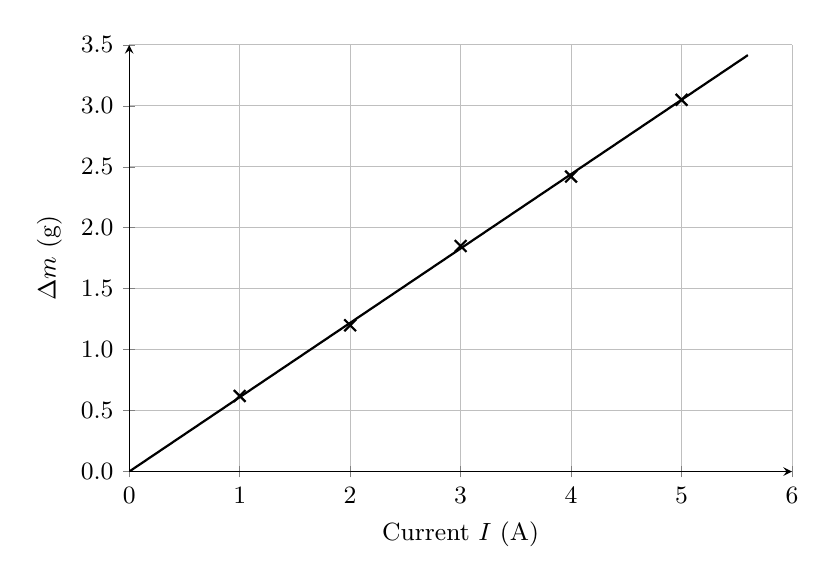
\begin{tikzpicture}
    \begin{axis}[width=100mm, height=70mm, axis lines=left, xmin=0, xmax=6, ymin=0, ymax=3.5,
        xtick={0,1,...,6}, ytick={0,0.5,...,3.5}, grid=major, major grid style={black!25},
        tick label style={font=\small}, label style={font=\small},
        yticklabel style={/pgf/number format/fixed, /pgf/number format/fixed zerofill, /pgf/number format/precision=1},
        xlabel={Current $I$ (\si{A})}, ylabel={$\Delta m$ (\si{g})},
        scaled ticks=false, enlargelimits=false]
      \addplot[only marks, mark=x, mark size=3pt, thick] coordinates {(1,0.62) (2,1.20) (3,1.85) (4,2.42) (5,3.05)};
      \addplot[line width=0.8pt, domain=0:5.6] {0.61*x};
    \end{axis}
  \end{tikzpicture}
\end{center}
\anspart{c}
\begin{crit}
  \critrow{Calculates the gradient from the line of best fit, relates it to $\frac{Bl}{g}$ AND
    calculates $B$ (accept 0.11 to \qty{0.13}{T})}{2}
  \critrow{Calculates the gradient OR states the relationship $\Delta m\,g = BIl$}{1}
\end{crit}
\sample
Using two widely spaced points on the line of best fit, $(0, 0)$ and $(5.6, 3.42)$:
gradient $= \dfrac{3.42 - 0}{5.6 - 0} \approx \qty{0.61}{g.A^{-1}} = \qty{6.1e-4}{kg.A^{-1}}$.
The extra force is $\Delta m\,g = BIl$, so the gradient is $\dfrac{Bl}{g}$:
\[ B = \frac{\text{gradient} \times g}{l} = \frac{(\num{6.1e-4})(9.8)}{0.050} = \qty{0.12}{T} \]

% ---- Q9
\ansq
\anspart{a}
\begin{crit}
  \critrow{Correctly calculates the current}{2}
  \critrow{Writes $BIl = mg$}{1}
\end{crit}
\sample
The tension is zero when the magnetic force balances the weight: $BIl = mg$, so
$I = \dfrac{mg}{Bl} = \dfrac{0.030 \times 9.8}{0.50 \times 0.20} = \qty{2.9}{A}$.
\anspart{b}
\begin{crit}
  \critrow{States from left to right (with the field into the page)}{1}
\end{crit}
\sample
The force must be upwards. With the field into the page, the current must flow from left to right
(palm rule: fingers into the page, thumb to the right, palm faces up).
\anspart{c}
\begin{crit}
  \critrow{States that the rod accelerates upwards (the acceleration is about $g$)}{1}
\end{crit}
\sample
The magnetic force doubles to $2mg$, so the net force is $mg$ upwards. The rod accelerates upwards at
\qty{9.8}{m.s^{-2}} (the leads go slack).

% ---- Q10
\ansq
\anspart{a}
\begin{crit}
  \critrow{Correctly calculates the force per metre AND states that it is repulsive}{2}
  \critrow{Correctly calculates the force per metre OR states repulsive with a reason}{1}
\end{crit}
\sample
$\dfrac{F}{l} = \dfrac{\mu_0 I_1 I_2}{2\pi r} = \dfrac{(4\pi\times10^{-7})(10)(10)}{2\pi(\num{3.0e-3})}
= \qty{6.7e-3}{N.m^{-1}}$. The current goes to the appliance in one conductor and back in the other, so
the currents are in opposite directions: the force is repulsive.
\anspart{b}
\begin{crit}
  \critrow{States that the force becomes four times as large, because both currents double}{1}
\end{crit}
\sample
Both conductors carry the same current, so $F \propto I^2$: doubling the current makes the force four
times as large (\qty{2.7e-2}{N.m^{-1}}).

% =====================================================================
\anstopic{Topic 3 - Electromagnetic Induction}

% ---- Q11
\ansq
\anspart{a}
\begin{crit}
  \critrow{Correctly calculates the change in flux}{1}
\end{crit}
\sample
$A = 0.080^2 = \qty{6.4e-3}{m^2}$; $\Delta\Phi = \Delta B \times A = 0.60 \times \num{6.4e-3} = \qty{3.8e-3}{Wb}$.
\anspart{b}
\begin{crit}
  \critrow{Correctly calculates the average emf}{2}
  \critrow{Uses $\varepsilon = N\frac{\Delta\Phi}{\Delta t}$ with correct values}{1}
\end{crit}
\sample
$\varepsilon = N\dfrac{\Delta\Phi}{\Delta t} = 50 \times \dfrac{\num{3.84e-3}}{0.30} = \qty{0.64}{V}$.
\anspart{c}
\begin{crit}
  \critrow{Correctly calculates the current}{1}
\end{crit}
\sample
$I = \dfrac{\varepsilon}{R} = \dfrac{0.64}{4.0} = \qty{0.16}{A}$.

% ---- Q12
\ansq
\begin{crit}
  \critrow{Sketches two pulses of opposite sign, with the second taller and narrower, AND explains the
    signs (Lenz's law) and the sizes (Faraday's law, faster magnet)}{4}
  \critrow{Sketches two pulses of opposite sign AND explains the signs or the sizes}{3}
  \critrow{Sketches two pulses of opposite sign, OR explains one feature}{2}
  \critrow{Gives one relevant point}{1}
\end{crit}
\sample
\begin{center}
  \begin{tikzpicture}
    \draw[axisline] (0,0) -- (5.2,0) node[right] {$t$};
    \draw[axisline] (0,-1.8) -- (0,1.9) node[above] {emf};
    \node[left, font=\small] at (0,0) {0};
    \draw[line width=1.1pt, domain=0:4.8, samples=150, smooth] plot (\x, {0.9*exp(-((\x-1.3)/0.42)^2) - 1.5*exp(-((\x-3.2)/0.25)^2)});
    \node[font=\scriptsize, align=center] at (1.3,1.25) {magnet\\entering};
    \node[font=\scriptsize, align=center] at (3.2,-1.95) {magnet leaving};
  \end{tikzpicture}
\end{center}
\begin{itemize}
  \item As the magnet enters, the flux through the coil increases, so an emf is induced (one sign).
  \item When the magnet is near the middle of the coil, the flux hardly changes, so the emf is about zero.
  \item As it leaves, the flux decreases, so the emf has the opposite sign (Lenz's law: the induced
        current always opposes the change in flux).
  \item The magnet speeds up as it falls, so the flux changes faster as it leaves: the second pulse is
        taller (Faraday's law, $\varepsilon = -N\frac{\Delta\Phi}{\Delta t}$) and shorter in time.
\end{itemize}

% ---- Q13
\ansq
\anspart{a}
\begin{crit}
  \critrow{Correctly states the turns ratio}{1}
\end{crit}
\sample
$N_\mathrm{p} : N_\mathrm{s} = V_\mathrm{p} : V_\mathrm{s} = 240 : 12 = 20 : 1$.
\anspart{b}
\begin{crit}
  \critrow{Correctly calculates the primary current}{2}
  \critrow{Uses $V_\mathrm{p}I_\mathrm{p} = V_\mathrm{s}I_\mathrm{s}$ (or the turns ratio)}{1}
\end{crit}
\sample
$V_\mathrm{p}I_\mathrm{p} = V_\mathrm{s}I_\mathrm{s}$, so
$I_\mathrm{p} = \dfrac{12 \times 6.0}{240} = \qty{0.30}{A}$.
\anspart{c}
\begin{crit}
  \critrow{Correctly calculates the primary current}{2}
  \critrow{Calculates the output power AND relates input and output power using the efficiency}{1}
\end{crit}
\sample
$P_\mathrm{out} = 12 \times 6.0 = \qty{72}{W}$. $P_\mathrm{in} = \dfrac{72}{0.90} = \qty{80}{W}$, so
$I_\mathrm{p} = \dfrac{80}{240} = \qty{0.33}{A}$.

% ---- Q14
\ansq
\begin{crit}
  \critrow{Explains TWO causes of energy loss AND describes a correct way to reduce each}{4}
  \critrow{Explains two causes and describes one way to reduce a loss}{3}
  \critrow{Identifies two causes, OR explains one cause and a way to reduce it}{2}
  \critrow{Gives one relevant point}{1}
\end{crit}
\sample
Any two of:
\begin{itemize}
  \item \textbf{Eddy currents:} the changing flux induces currents in the iron core, which heat it.
        Reduce them by making the core from thin, insulated laminations (or ferrite), which breaks up the
        current paths.
  \item \textbf{Resistive heating of the coils:} the currents heat the copper wires ($P = I^2R$).
        Reduce this by using thick, low-resistance copper wire (and cooling the transformer).
  \item \textbf{Incomplete flux linkage:} some of the flux from the primary coil does not pass through
        the secondary coil. Reduce this by winding both coils on the same closed soft-iron core, or one on
        top of the other.
  \item \textbf{Hysteresis in the core:} energy is lost each time the core is magnetised in one direction
        and then the other. Reduce this by using a soft-iron (easily magnetised) core.
\end{itemize}

% ---- Q15
\ansq
\anspart{a}
\begin{crit}
  \critrow{Correctly calculates the power loss for both voltages}{3}
  \critrow{Correctly calculates the power loss for one voltage (or both currents)}{2}
  \critrow{Calculates one current OR uses $P = I^2R$}{1}
\end{crit}
\sample
At \qty{2.0}{kV}: $I = \dfrac{P}{V} = \dfrac{\num{200e3}}{\num{2.0e3}} = \qty{100}{A}$;
loss $= I^2R = 100^2 \times 0.50 = \qty{5.0e3}{W}$ (2.5\% of the power).\\
At \qty{20}{kV}: $I = \qty{10}{A}$; loss $= 10^2 \times 0.50 = \qty{50}{W}$ (0.025\%).
\anspart{b}
\begin{crit}
  \critrow{Explains the step-up transformer (high voltage, low current, low $I^2R$ loss) AND the
    step-down transformer (safe, usable voltage)}{2}
  \critrow{Explains one of these}{1}
\end{crit}
\sample
A step-up transformer at the power station raises the voltage, so the same power is sent with a much
smaller current and the $I^2R$ loss is much smaller (100 times smaller for 10 times the voltage, as in
part (a)). A step-down transformer near the users lowers the voltage to a safe level that appliances
can use (\qty{240}{V}).

% =====================================================================
\anstopic{Topic 4 - Applications of the Motor Effect}

% ---- Q16
\ansq
\anspart{a}
\begin{crit}
  \critrow{Correctly calculates the maximum torque}{2}
  \critrow{Calculates the area OR uses $\tau = nIAB$}{1}
\end{crit}
\sample
$A = 0.050 \times 0.040 = \qty{2.0e-3}{m^2}$. The torque is greatest when the plane of the coil is
parallel to the field: $\tau = nIAB = 200 \times 1.5 \times \num{2.0e-3} \times 0.35 = \qty{0.21}{N.m}$.
\anspart{b}
\begin{crit}
  \critrow{Explains why the torque varies ($\tau = nIAB\sin\theta$; maximum when the plane is parallel to
    the field, zero when it is at right angles) AND explains that the commutator reverses the current
    every half turn so the torque keeps the same direction}{3}
  \critrow{Explains the variation of torque OR the role of the commutator}{2}
  \critrow{Gives one relevant point}{1}
\end{crit}
\sample
The forces on the sides of the coil stay the same size, but as the coil turns, their perpendicular
distance from the axis changes: $\tau = nIAB\sin\theta$, where $\theta$ is the angle between the field
and the normal to the coil. The torque is greatest when the plane of the coil is parallel to the field
and zero when it is at right angles to the field. If the current stayed the same, the torque would
reverse after this position and the coil would rock back and stop. The split-ring commutator reverses the
current in the coil every half turn, just as the coil passes this position, so the torque always acts in
the same direction and the motor keeps turning.

% ---- Q17
\ansq
\anspart{a}
\begin{crit}
  \critrow{Correctly calculates the starting current}{1}
\end{crit}
\sample
At the start the motor is not turning, so there is no back emf: $I = \dfrac{V}{R} = \dfrac{12}{1.5} = \qty{8.0}{A}$.
\anspart{b}
\begin{crit}
  \critrow{Correctly calculates the back emf}{2}
  \critrow{Uses $V = \varepsilon_\mathrm{back} + IR$}{1}
\end{crit}
\sample
$V = \varepsilon_\mathrm{back} + IR$, so $\varepsilon_\mathrm{back} = 12 - 1.2 \times 1.5 = \qty{10.2}{V}$.
\anspart{c}
\begin{crit}
  \critrow{Explains that a jammed motor produces no back emf, so the current stays large, causing large
    $I^2R$ heating}{2}
  \critrow{Gives one relevant point}{1}
\end{crit}
\sample
A jammed motor does not turn, so no back emf is produced. The current stays at its large starting value
($\frac{V}{R} = \qty{8.0}{A}$), and the heating in the coil ($I^2R = \qty{96}{W}$, compared with about
\qty{2}{W} when running) can melt the insulation and burn out the motor.

% ---- Q18
\ansq
\begin{crit}
  \critrow{Compares the structure (slip rings vs split-ring commutator) AND the output (AC vs pulsating
    DC), explaining how the structure causes the difference}{4}
  \critrow{Compares structure and output with a minor omission}{3}
  \critrow{Describes the structure OR the output of each}{2}
  \critrow{Gives one relevant point}{1}
\end{crit}
\sample
Both have a coil that is turned in a magnetic field, and brushes that connect the coil to the external
circuit; in both, the emf in the coil alternates as it turns. In an AC generator each end of the coil is
connected to its own slip ring, so the connections never swap and the output alternates (a sine-shaped
voltage that changes direction every half turn). In a DC generator the coil is connected through a
split-ring commutator, which swaps the connections every half turn, so the output always has the same
direction: a pulsating DC, like a sine curve with the negative halves turned up.

% ---- Q19
\ansq
\begin{crit}
  \critrow{Explains the rotating field of the stator, the induced currents in the rotor, AND the force
    on the rotor (motor effect / Lenz's law) that drags it after the field}{4}
  \critrow{Explains most of these steps}{3}
  \critrow{Describes some features of the motor}{2}
  \critrow{Gives one relevant point}{1}
\end{crit}
\sample
AC in the stator coils produces a magnetic field that rotates around the motor. The rotor (a squirrel
cage of conducting bars joined by end rings) is in this field. Because the field moves relative to the
bars, the flux through the rotor changes, so emfs and currents are induced in the bars (Faraday's law).
These currents are in the magnetic field, so forces act on them (motor effect), producing a torque. By
Lenz's law the forces oppose the relative motion, so they drag the rotor round after the rotating field.
The rotor always turns a little slower than the field (slip); if it turned at the same speed, there would
be no induced current and no torque.

% ---- Q20
\ansq
\begin{crit}
  \critrow{Explains the induced eddy currents, the opposing force (Lenz's law), the energy
    transformation (kinetic energy to heat) linked to conservation of energy, AND why the force
    decreases as the speed decreases}{5}
  \critrow{Explains most of these points}{4}
  \critrow{Explains eddy currents and the opposing force, OR the energy transformation}{3}
  \critrow{Describes some relevant features}{2}
  \critrow{Gives one relevant point}{1}
\end{crit}
\sample
As each copper fin moves between the magnets, the magnetic flux through parts of the fin changes, so
emfs and eddy currents are induced in the fin (Faraday's law). By Lenz's law the eddy currents produce
magnetic fields that oppose the change that caused them, so there is a force on the fin that opposes its
motion through the magnets: a braking force, with no contact.

Energy is conserved: the kinetic energy of the cars is changed into the electrical energy of the eddy
currents, which is then changed into heat in the copper ($I^2R$). Lenz's law follows from this: if the
induced currents helped the motion, the cars would speed up and gain energy from nothing.

The induced emf depends on the rate of change of flux, which is proportional to the speed of the fins.
As the cars slow down, the eddy currents and the braking force become smaller, so the braking is smooth,
but it cannot hold the cars still; friction brakes are needed to stop them completely.

\end{document}
